\chapter{Introduction}\label{ch:introduction}

\section{Introduction}

An electrocardiogram (ECG) records the small voltage changes that occur when
electrical activity moves through the heart. Electrodes on the body see this
activity from different directions. In an ECG trace, the horizontal axis shows
time and the vertical axis shows voltage. ECG analysis is useful because the
pattern changes when a heartbeat starts in a different place, happens at a
different time, or travels through the heart in a different way.

\textbf{Components of one ECG beat.}
A normal heartbeat starts when the sinoatrial node creates an impulse. The
P wave shows atrial depolarisation. The short, sharp QRS complex mainly shows
ventricular depolarisation. The T wave shows ventricular repolarisation. The
time between two neighbouring R peaks is called the RR interval. It gives
information about heart rate and rhythm regularity
\cite{kligfield2007standardization}. Figure~\ref{fig:intro-ecg-anatomy} shows
these parts in a simple way. In real recordings, the same beat can look
inverted, stretched, or noisy because of the lead, the patient, the electrodes,
and the recording conditions.

\begin{figure}[H]
\centering
\begin{tikzpicture}[x=1.15cm,y=1.15cm,font=\small,>=latex]
\draw[->,draw=thesisslate] (0,0)--(12.2,0) node[right]{time};
\draw[->,draw=thesisslate] (0,-1.25)--(0,2.15)
  node[above,align=center]{ECG\\voltage};
\draw[thesisteal,very thick,line join=round]
  plot[smooth] coordinates {
  (0.2,0) (1.0,0) (1.35,.10) (1.65,.34) (1.95,.10) (2.3,0)
  (3.15,0) (3.38,-.20) (3.55,1.85) (3.72,-.60) (4.0,.12) (4.35,0)
  (5.25,0) (5.75,.18) (6.25,.62) (6.75,.18) (7.2,0) (8.0,0)
  (8.35,.10) (8.65,.33) (8.95,.10) (9.30,0)
  (10.15,0) (10.38,-.20) (10.55,1.85) (10.72,-.60) (11.0,.12) (11.35,0)};
\node[text=black,font=\bfseries] at (1.65,.65) {P};
\node[text=black,font=\bfseries] at (3.28,-.52) {Q};
\node[text=black,font=\bfseries] at (3.86,2.02) {R};
\node[text=black,font=\bfseries] at (3.75,-.92) {S};
\node[text=black,font=\bfseries] at (6.25,.92) {T};
\draw[<->,thick,draw=orange!80!black] (3.55,-1.05)--(10.55,-1.05)
  node[midway,fill=white,inner sep=2pt]{RR interval};
\draw[decorate,decoration={brace,amplitude=5pt},draw=thesisnavy]
  (3.18,1.55)--(3.88,1.55);
\node[anchor=east,text=black] at (3.18,1.78) {QRS complex};
\end{tikzpicture}
\caption{Main components of a simplified ECG beat. Shape features describe the
P--QRS--T pattern, while RR features describe timing between beats. This is an
educational drawing, not a diagnostic template.}
\label{fig:intro-ecg-anatomy}
\end{figure}

\textbf{Arrhythmia and the classes considered.}
An arrhythmia is a problem in where the heart's electrical activity starts,
when it happens, how it is ordered, or how it travels. It may affect one beat,
many repeated beats, or a longer rhythm. This study uses one normal output and
five arrhythmia outputs. Table~\ref{tab:intro-arrhythmias} summarises the main
physiological cause and visible ECG behaviour for each one. These descriptions
define the model task only. A clinical diagnosis still needs the full ECG and
patient context \cite{moody2001impact,dechazal2004heartbeat}.

\begin{table}[H]
\centering
\small
\caption{Normal rhythm and the five arrhythmia types considered in this study.}
\label{tab:intro-arrhythmias}
\begin{tabular}{>{\raggedright\arraybackslash}p{2.2cm}>{\raggedright\arraybackslash}p{5.0cm}>{\raggedright\arraybackslash}p{5.4cm}}
\toprule
Type & Main reason & Typical ECG behaviour and importance\\
\midrule
Normal sinus rhythm (N) & The impulse begins in the sinoatrial node and follows
the normal conduction path. & Repeated P--QRS--T patterns and generally regular
RR intervals. It supplies the reference against which unusual beats are
compared.\\
PVC & A premature impulse begins in a ventricle instead of following the normal
path from the atria. & The beat occurs early and often has a wide, unusual QRS,
followed by a pause. Detection is important because it is a clear ventricular
abnormality and can occur repeatedly.\\
PAC & A premature impulse begins in an atrial location outside the sinoatrial
node. & The beat occurs early; the P wave may change, while the QRS can remain
narrow and similar to normal. Its subtle shape makes PAC difficult to separate
from normal beats.\\
LBBB & Electrical conduction through the left bundle branch is delayed or
blocked. & The ventricles activate in an altered sequence, producing a broad,
changed QRS. Recognition is important because the pattern can be associated
with underlying cardiac disease.\\
RBBB & Electrical conduction through the right bundle branch is delayed or
blocked. & The later part of the QRS changes and can show a second peak in some
leads. It must be separated from LBBB because the delayed side is different.\\
AFib & Atrial electrical activity becomes rapid and disorganised rather than
following one regular atrial impulse. & Consistent P waves disappear and RR
intervals become irregular. Identification is important because AFib is linked
with clinically important complications and requires rhythm-level evidence.\\
\bottomrule
\end{tabular}
\end{table}

Figure~\ref{fig:intro-real-arrhythmias} shows real labelled ECG segments from
the MIT--BIH Arrhythmia Database instead of drawings. Each panel comes from the
fixed final 20\% of its record. For each stated record and class, the displayed
window is the one closest to that held-out group's mean waveform by squared
distance. This rule gives a representative example without choosing the most
dramatic-looking beat. The signals were resampled to 128 Hz, standardised, and
aligned so the labelled R peak is at 1.5625 seconds.

\begin{figure}[H]
\centering
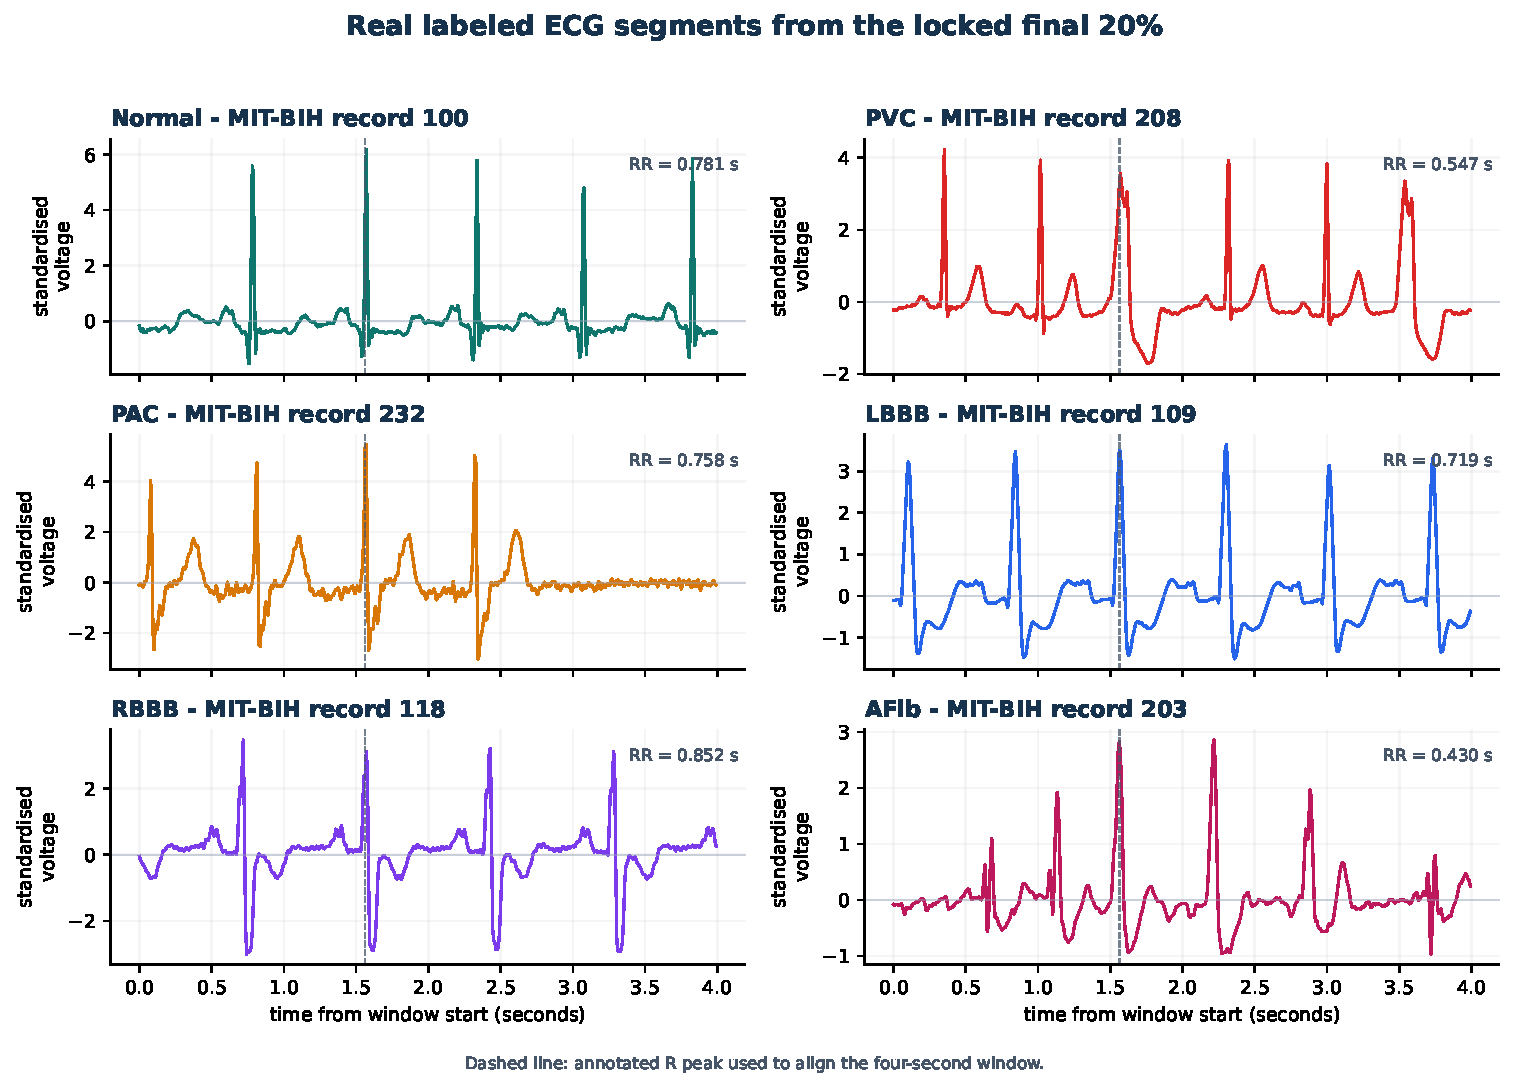
\includegraphics[width=.99\textwidth]{pic/generated/real_arrhythmia_examples.pdf}
\caption{Real four-second ECG examples from the MIT--BIH Arrhythmia Database:
normal record 100, PVC record 208, PAC record 232, LBBB record 109, RBBB record
118, and AFib record 203. The dashed line marks the annotated central R peak.
The examples are used for explanation and are not clinical diagnostic
templates.}
\label{fig:intro-real-arrhythmias}
\end{figure}

These examples show why one simple threshold is not enough. PVC, LBBB, and RBBB
mainly change beat shape. PAC can occur early while still looking close to a
normal beat. AFib is often clearer from changing intervals and rhythm context.
For this reason, the final system combines MLII waveform shape, frequency
information, RR history, and disagreement with a learned normal reconstruction.

Finding these patterns matters because long ECG recordings can contain too many
beats for continuous manual review. An automated research system can mark
suspicious regions, count events, and help a reviewer focus attention. At the
same time, an error can miss an abnormality or create an unnecessary alarm.
Therefore, accuracy, per-class recall, confidence intervals, and clear limits
are all needed. The system developed here is for research evaluation only. It
is not a replacement for a clinician.

\section{Research Problem}

The central research problem is stated below.

\begin{tcolorbox}[
  colback=thesislight,
  colframe=thesisteal,
  boxrule=.8pt,
  arc=3pt,
  left=6pt,right=6pt,top=6pt,bottom=6pt
]
\textbf{Main research problem:} How can an explainable two-stage ECG system use
normal-only reconstruction, beat morphology, and heartbeat timing to detect
abnormal beats and correctly identify PVC, PAC, LBBB, RBBB, and AFib with more
than 90\% whole-system accuracy on a fixed temporal test, while providing
statistically valid evidence across patients?
\end{tcolorbox}

The main problem contains four connected sub-problems:
\begin{enumerate}
    \item ECG shape varies between patients and leads, so harmless personal
    morphology can resemble an abnormality.
    \item A two-stage system can fail at the abnormality gate or at subtype
    classification; a missed abnormal beat never reaches the second stage.
    \item Normal and arrhythmia classes have unequal numbers of beats and
    patients, so ordinary accuracy can hide failure on a rare class.
    \item Thousands of neighbouring beats from one patient are correlated.
    Testing must keep the final signal unseen and must calculate uncertainty
    using complete patient clusters rather than treating beats as independent
    people.
\end{enumerate}

The final experiment handles these problems with a chronological split. The
first 64\% of each MITDB record trains candidate models, the next 16\% selects
the models and threshold, and the final 20\% is reserved for temporal testing.
The present model fitting excludes test rows, but the segment was observed
during earlier development. Percentages count accepted beats in chronological
order, rather than exact recording duration. The result is therefore a
retrospective patient-adapted temporal evaluation, with possible selection
optimism and no confirmatory claim about completely new patients.

\section{Objective and Expected Outcomes}

\textbf{Main objective.}
The main objective is to develop and statistically evaluate an ECG
system that first detects abnormal beats and then identifies five supported
arrhythmia types in later unseen signal from known patients.

\textbf{Specific objectives.}
\begin{enumerate}
    \item Train a normal-only autoencoder with the complete first ECG channel
    from all 18 MIT--BIH Normal Sinus Rhythm Database subjects and use its
    reconstruction errors as evidence.
    \item Use the earlier 80\% of every MITDB record containing MLII for
    supervised development while keeping every final 20\% portion unavailable.
    \item Build a binary abnormality detector using ECG morphology, spectrum,
    RR timing, and autoencoder-residual features;
    \item Build a second classifier for PVC, PAC, LBBB, RBBB, and AFib using
    the same MLII signal and RR context with a next-beat delay;
    \item measure abnormality-detection accuracy, conditional subtype accuracy,
    and complete six-class system accuracy separately;
    \item report the true and correctly classified count for every arrhythmia;
    and
    \item validate uncertainty with equal-subject accuracy, a complete-subject
    bootstrap confidence interval, and subject-level statistical tests.
\end{enumerate}

\textbf{Expected outcomes.}
The planned outcomes are:
\begin{itemize}
    \item a reproducible, deployable two-stage research prototype;
    \item abnormality-detection, subtype, and whole-system point accuracies
    above 90\% on the fixed temporal test;
    \item a whole-system 95\% confidence interval whose lower bound exceeds
    90\% and whose total width is no more than three percentage points;
    \item per-arrhythmia results that reveal whether every supported class
    reaches the accuracy target; and
    \item an honest statement of the data, statistical, hardware, and clinical
    limits of the model.
\end{itemize}

These are evaluation targets, not assumed conclusions. Chapter~\ref{ch:results}
reports which targets were reached and which were not.

\section{Research questions}
\begin{description}
\item[RQ1] How does the frozen NSRDB reconstruction branch contribute evidence
to the supervised hierarchy, and has its independent benefit been measured?
\item[RQ2] What are binary, conditional-subtype, and complete six-class
performance on the retrospective temporal evaluation?
\item[RQ3] What do equal-subject accuracy and subject-clustered uncertainty
show about variation across known patients?
\item[RQ4] Do the measured accuracy, interval precision, and class recalls
meet the study targets, and what evidence exists for external use?
\end{description}

The labels PVC, PAC, N and AFib are operational annotation groups defined in
Chapter~\ref{ch:data}; AFib includes flutter. A successful software
implementation is distinct from meeting every statistical target.
